\chapter{Design}
\label{sec:design}

% Ist das zentrale Kapitel der Arbeit. Hier werden das Ziel sowie die
% eigenen Ideen, Wertungen, Entwurfsentscheidungen vorgebracht. Es kann
% sich lohnen, verschiedene Möglichkeiten durchzuspielen und dann
% explizit zu begründen, warum man sich für eine bestimmte entschieden
% hat. Dieses Kapitel sollte - zumindest in Stichworten - schon bei den
% ersten Festlegungen eines Entwurfs skizziert werden.
% Es wird sich aber in einer normal verlaufenden
% Arbeit dauernd etwas daran ändern. Das Kapitel darf nicht zu
% detailliert werden, sonst langweilt sich der Leser. Es ist sehr
% wichtig, das richtige Abstraktionsniveau zu finden. Beim Verfassen
% sollte man auf die Wiederverwendbarkeit des Textes achten.

% Plant man eine Veröffentlichung aus der Arbeit zu machen, können von
% diesem Kapitel Teile genommen werden. Das Kapitel wird in der Regel
% wohl mindestens 8 Seiten haben, mehr als 20 können ein Hinweis darauf
% sein, daß das Abstraktionsniveau verfehlt wurde.

%\ldots design \ldots

%\todo{write design}






% \section{Recap}

% \subsection{k8s overview}

%     \begin{figure}[H]
%         \centering
%         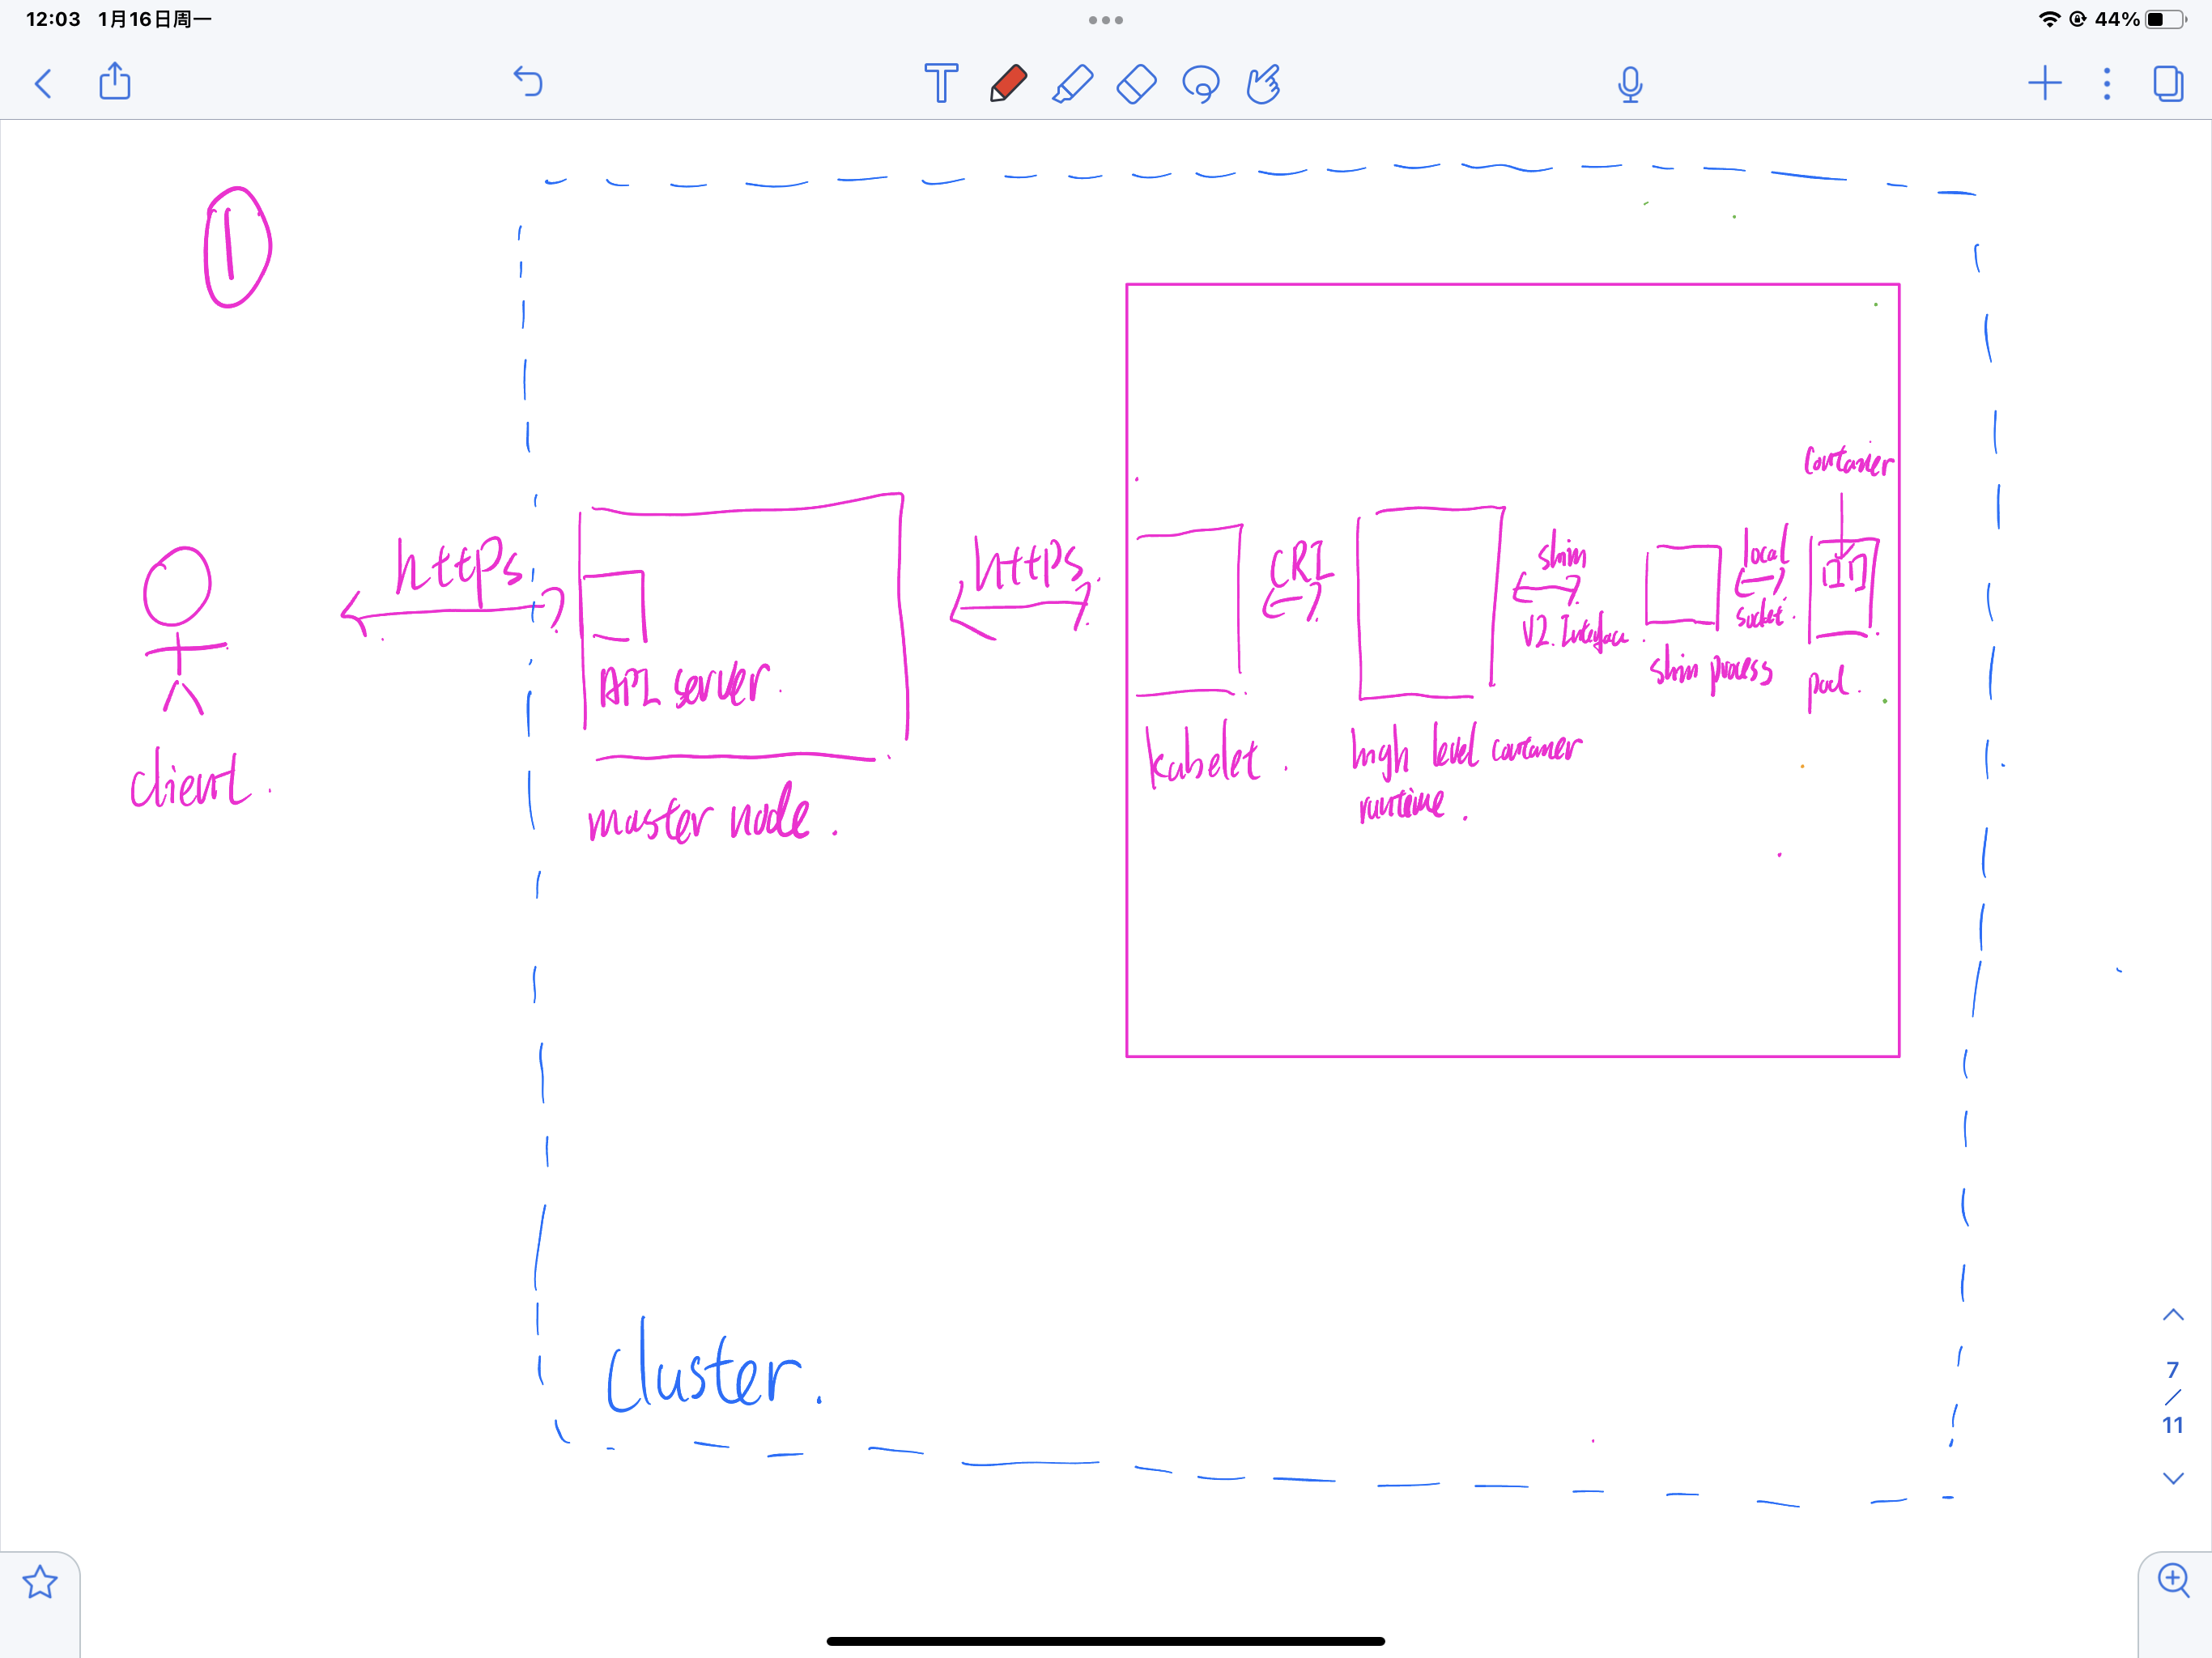
\includegraphics[width=0.8\textwidth]{images/IMG_4416.PNG}
%         \caption[k8s arch]{k8s arch}
%         \label{fig:k8s}
%     \end{figure}

%     The tenant connects to the api server located on the master node via the https protocol and issues commands to the cluster via this channel
    
%     The master node establishes a connection to the kubelet service located on each worker node via the https protocol. Through this channel, it can manage the lifecycle of the worker nodes and the pods running on them. Furthermore, commands sent from the tenant to the master node 
%     are also sent to the worker nodes through this link, including creating a pod, deleting a pod, etc.
    
%     The kubelet at each worker node acts as an agent, listening for requests/commands from the master and calling other services located on the same node to fulfill the request.
    
%     In the case of container/image management related requests, it makes a call to a host choosed high level container runtime.
%     These High-level container managers, such as containerd, and cri-o, are responsible for managing the container lifecycle and images, while the actual creation/deletion of pods/containers is done by the lower-level container runtime or so called shim process.

%     Furthermore, it is worth noting that in order to facilitate communication between kubelet and different high level container runtimes, kubelet proposes an abstract interface called CRI interface. This interface defines a set 
%     of endpoints for how high levek container runtime manage the lifecycle of pods/containers and images. Therefore, it must be implemented by any high-level container runtime that wishes to integrate into the k8s environment. This interface breaks the dependency between kubelet 
%     and a specific high-level container manager and greatly improves the extensibility of k8s.
    
%     Similar to the idea of defining a CRI interface, the high-level container runtime also defines an abstract interface for communicating with shim processes that run containers in different ways. In the case of containerd, this abstract interface is called the shim v2 API. 
%     This interface defines endpoints for creating/deleting containers, issuing commands to a container or allocating terminal in a container etc.


% \subsection{quark overview}


% \begin{figure}[H]
%     \centering
%     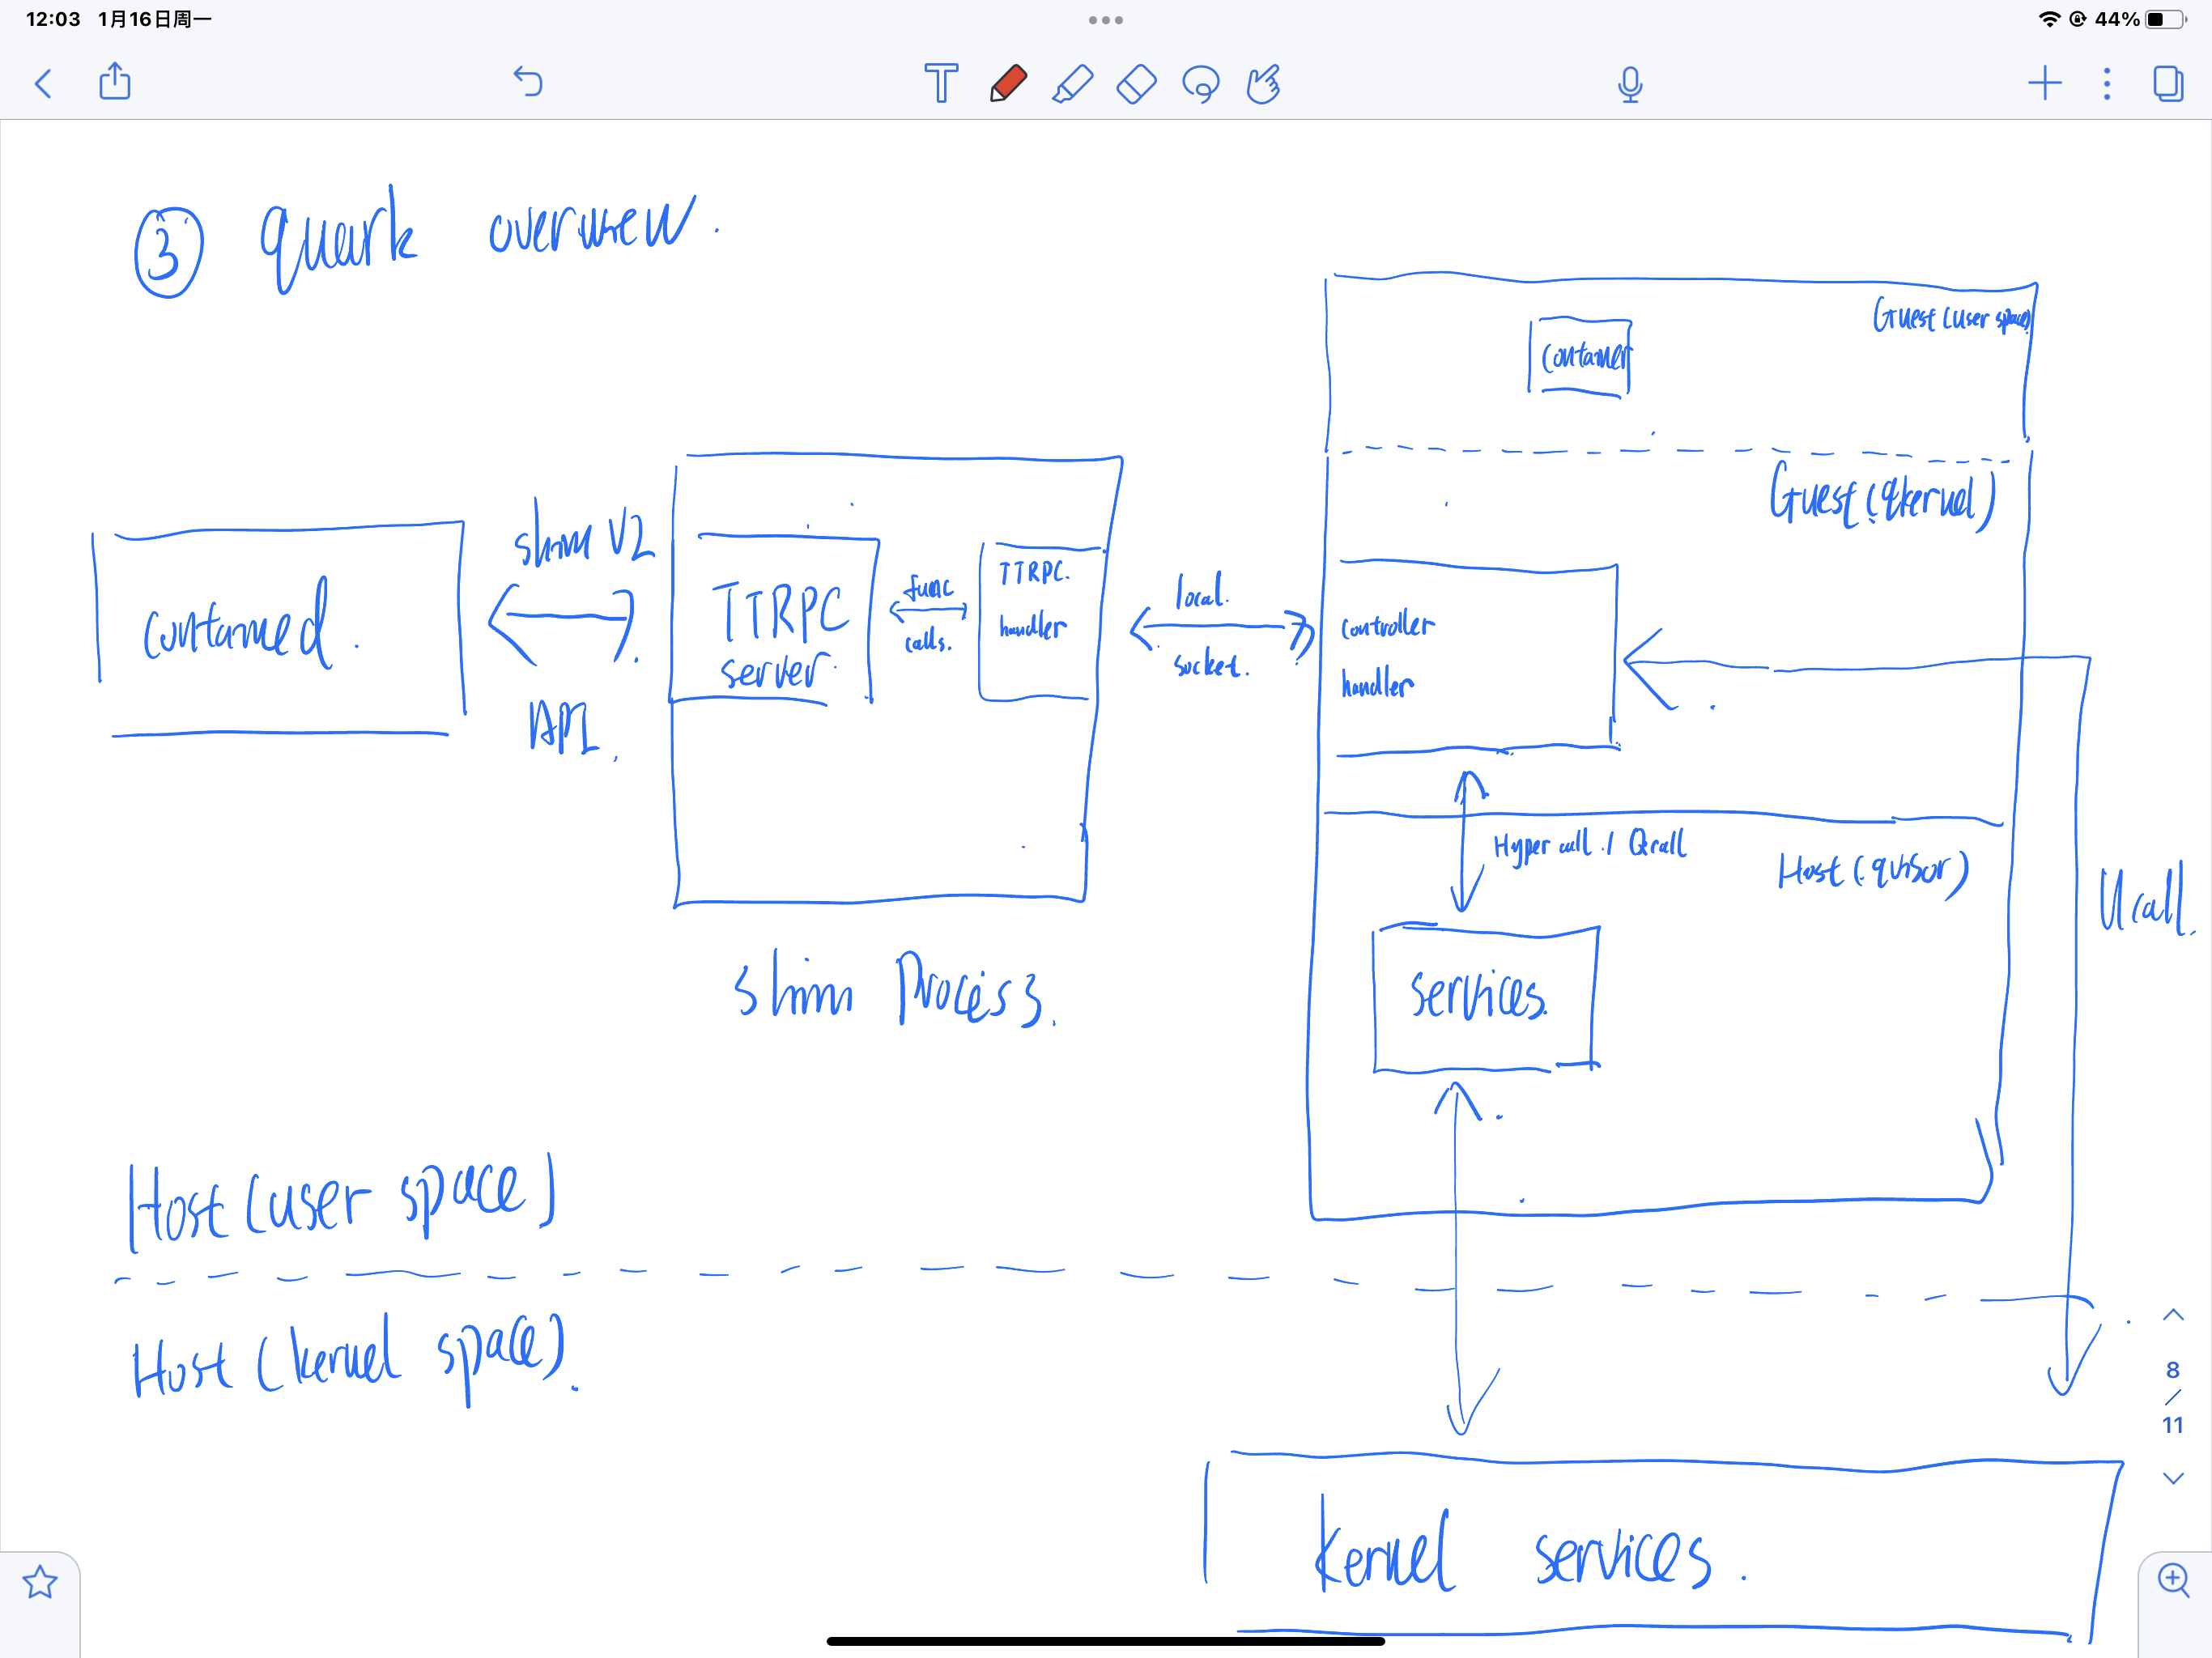
\includegraphics[width=0.8\textwidth]{images/IMG_4415.PNG}
%     \caption[quark]{quark}
%     \label{fig:quark}
% \end{figure}
% In this section, we introduce the components that constitute quark runtime, and how quark is integrated into the k8s ecosystem.

% As we can see from the diagram, quark runtime consists of three main components.
% \begin{itemize}
%     \item  shim process: The shim process is a qvisor binary that is started by containerd. Since containerd executes this binary with the shim keyword as a program argument, The process that executes this binary enters shim mode. This process  is therefore also called the shim process. The shim process starts a ttrpc server as a means of communication with cotnainerd, which implements the endpoints defined in the containerd shim v2 API. Therefore, containerd can send commands to the ttrpc server to inform the shim process to complete the appropriate operations, including creating, deleting a container, etc.
%     \item  qvisor (VMM) and qkernel: qkernel and qvisor belong to the same process on the right side of the graph. Similar to the relationship between qemu and the guest Linux operating system, qvisor acts as a virtual machine manager and is responsible for providing various services to the guest OS qkernel, such as IO emulation, system call emulation, etc., while qkernel is responsible for managing the guest processes, preparing the file system for the guest processes, etc.
% \end{itemize}
% As we mentioned in the previous section, when cri-plugin get a container creation command from kubelet, it first sends a create pod command to the shim process and let the shim process to create a special 
% pause container as a sandbox container. In the case of the quark runtime, the shim process spawns a subprocess to execute the qvisor binary. This qvisor subprocess first creates a virtual 
% machine with the qkernel as the guest operating system, then informs the qkernel to start this pause container and starts a socket server "controller hander" as a means of communication with 
% the shim process. Then, shim sends start application container request to "controller hander", and passes the metadata related to the container to qkernel, 
% which will then start the application container based on the metadata.

% Qkernel has 2 path to access the external services (services provided by qvisor/kernel)
% \begin{itemize}
%     \item  Ucall path (fast path): please see section \ref*{Qcall_hypercall_ucall}
%     \item  Qcall/ Hyper call (slow path): please see section \ref*{Qcall_hypercall_ucall}
% \end{itemize}

\section{Overview of confidential quark in cloud environments}
\begin{figure}[H]
    \centering
    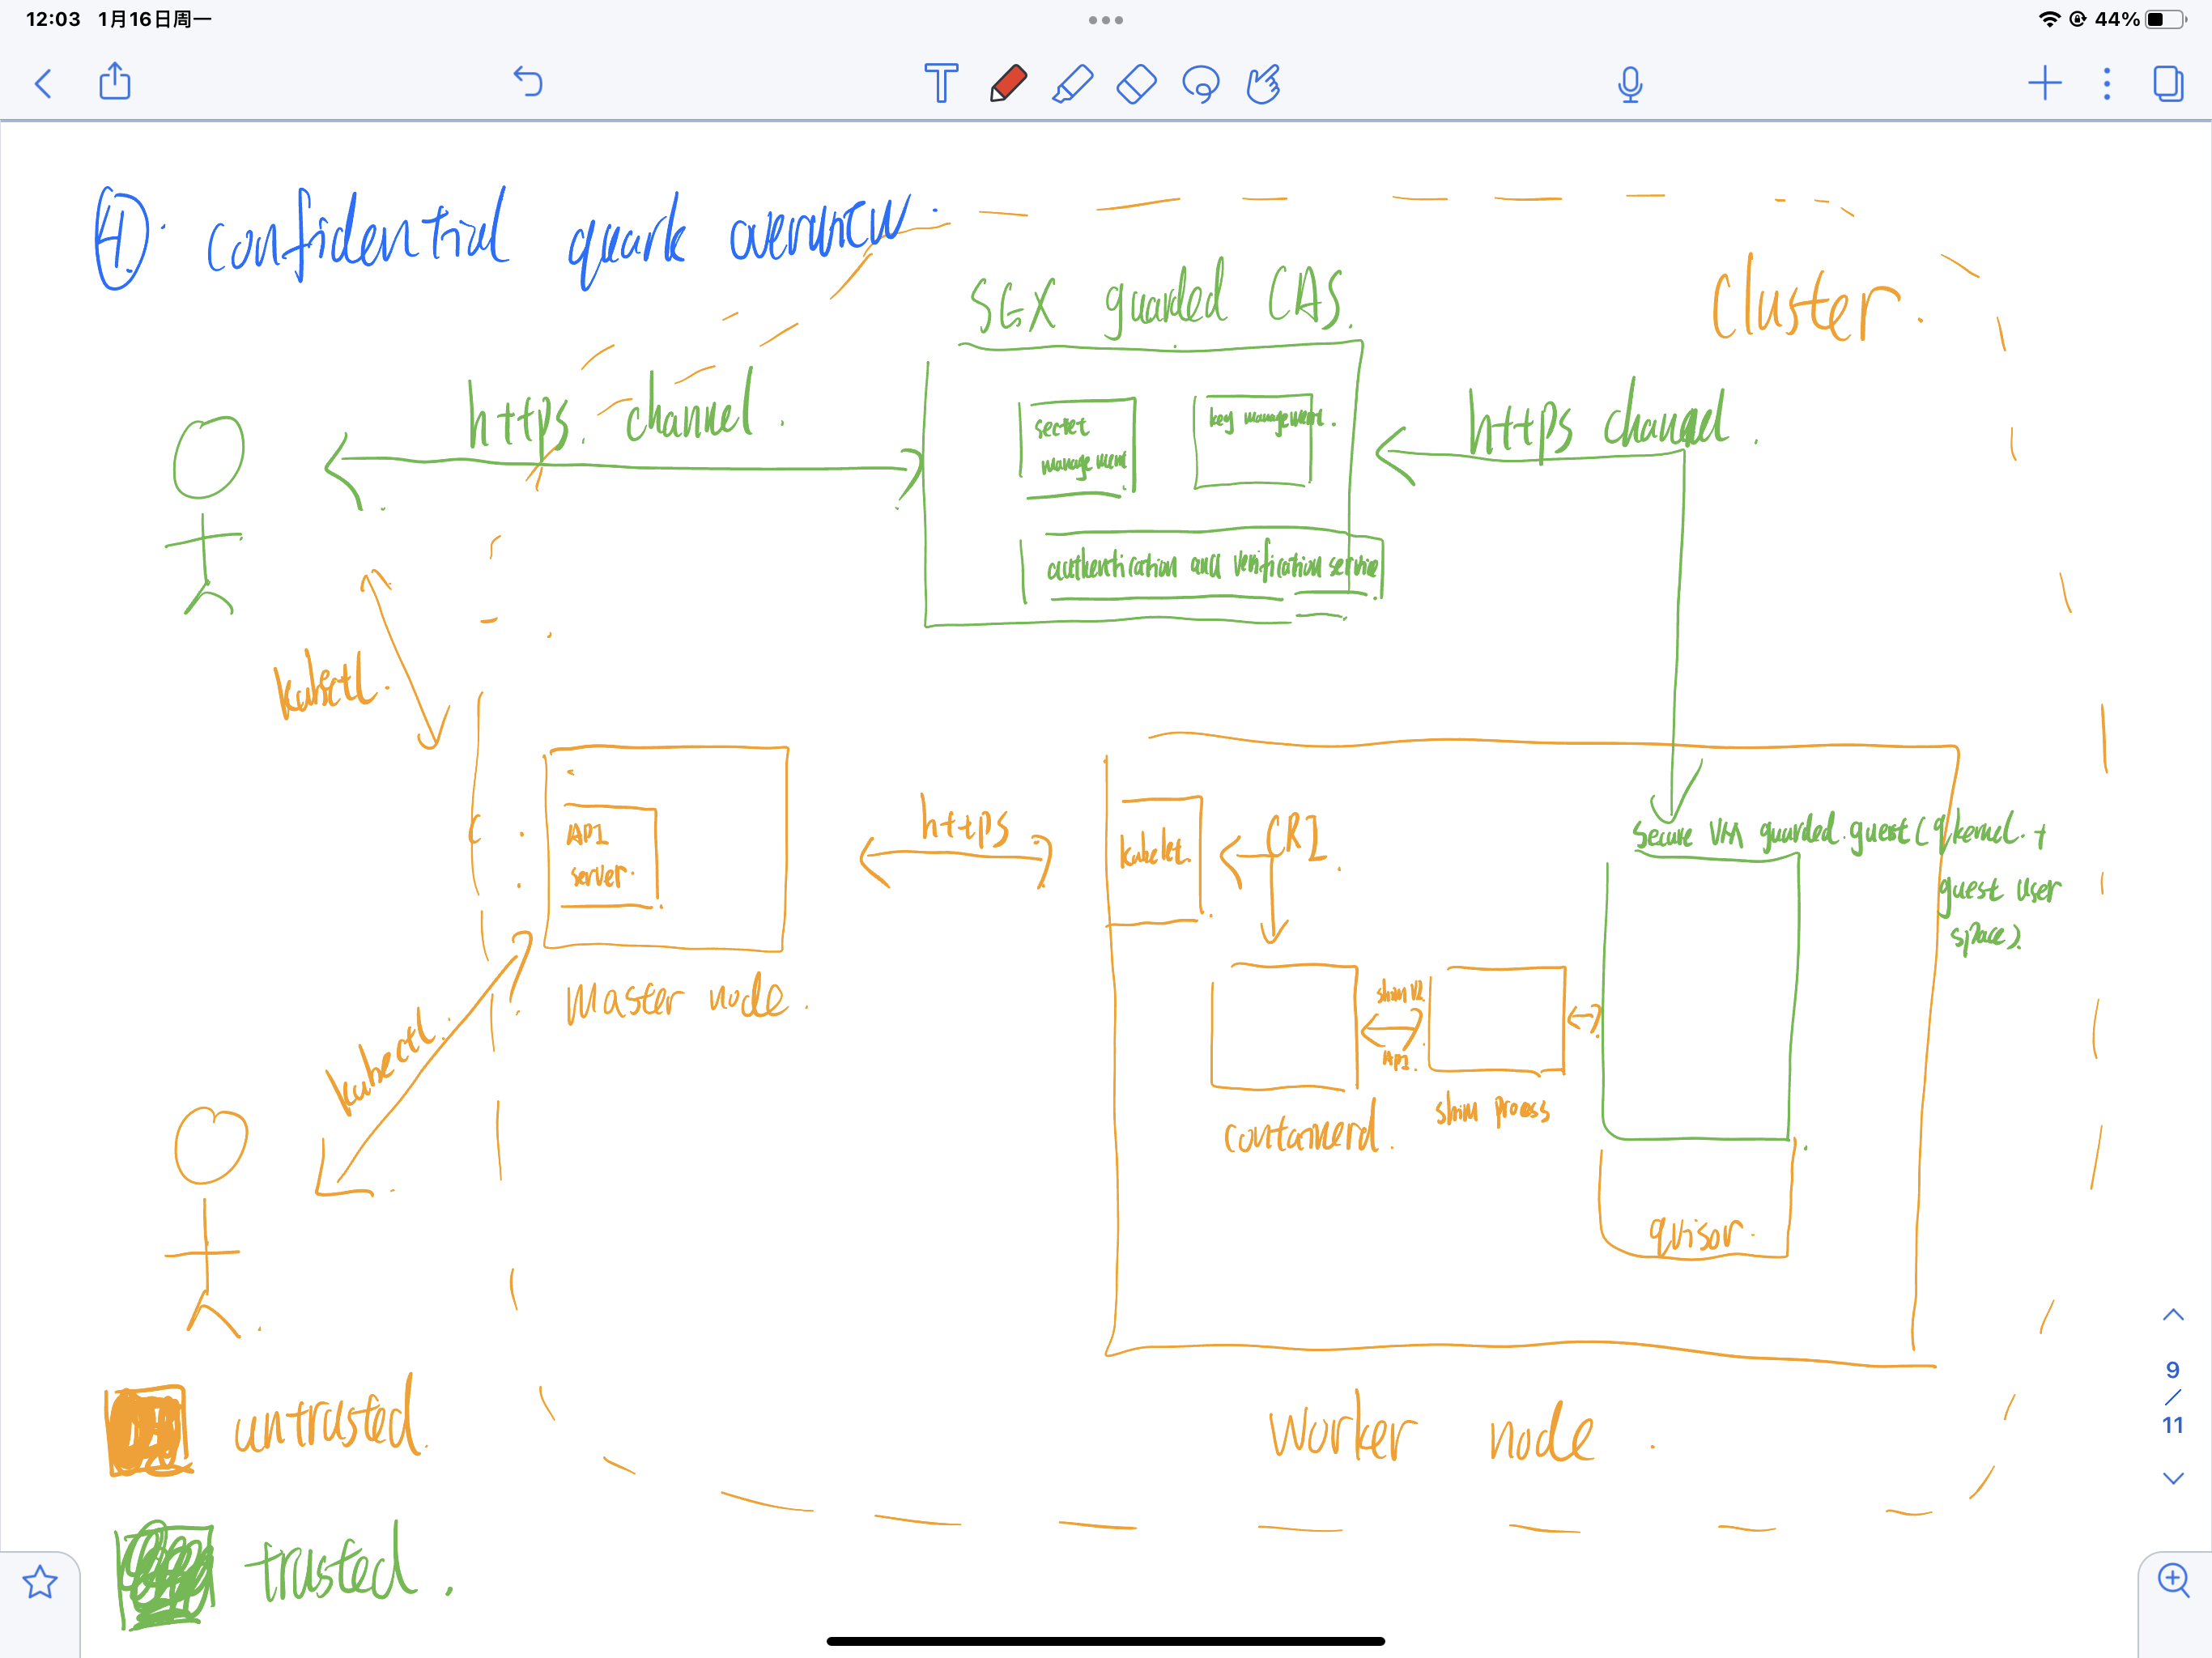
\includegraphics[width=0.8\textwidth]{images/IMG_4414.PNG}
    \caption[confidential quark]{confidential quark}
    \label{fig:confidential_quark}
\end{figure}
In this section, we describe the components that make up a confidential quark, and the cloud infrastructure required to support remote attestation, and secret provisioning.
In the figure, we divide the components of the cluster into trusted and untrusted components, where the trusted components are in green ,which includes CAS and qkernel running in trusted VMs, and the other components in orange are untrusted.

CAS running in a HW based TEE is a trusted component that manages data owner uploaded secrets and policies, authenticates the qkernel, and makes secrets available to qkernel in a secure manner. Data owners can verify that CAS is trusted by means of remote attestation, before uploading the secrets required by the application container and the policy required by the qkernel shield to the CAS via tls channel.

The qkernel, which serves as the guest operating system, is protected by a secure virtual machine along with the application container process running in the guest user space. In this case, the guest's memory and the cpu registers being used are encrypted. Consequently, entities running outside of the guest, such as qvisor, cotnainerd, cannot view the contents of the guest.
In the following, for simplicity, we refer to the SVM-protected qkernel and application container uniformly as the confidential qkernel. 

The confidential qkernel also allows remote entities, in our case, the CAS, to attests against it dynamicly. This is achieved by the confidential qkernel sending its remote attestation report to CAS. 
This report is typically generated by the SVM running the confidential qkernel and contains a set of measurements about the confidential qkernel. With the help of hardware vendor's remote attestation infrastructure, CAS can determine that the 
confidential qkernel is running in an expected environment.

We delegate the deployment and management of the confidential quark to an untrusted entity, the "cloud operator," i.e., the orange villain in the lower left corner of the diagram. The cloud operator can deploy confidential quarks using 
common kubectl commands or yaml files. The difference from deploying a legacy workload is that when deploying a confidential quark, the cloud operator needs to pass 
the IP address of the CAS as an environment variable to the confidential quark, and later the shield running inside a confidential quark will use this IP address to find the CAS and complete the remote attestation and secret injection. We elaborate on the process of secure deployment in the next section.

Delegating the management of the confidential quark may compromise the confidentiality of the container running in it.  An obvious example is the kubectl exec endpoint. With this endpoint, one can issue any command to a container running in the confidential qkernel. 
When the qkernel receives the command, the qkernel starts a guest user level process to execute a binary corresponding to the command. Since the access to memory ,registers, and files from inside the SVM is in plaintext, the process can easily obtain 
the secrets held by the confidential qkernel and return them to the cloud operator. We address this problem by defining the permissions for each role in the cluster, following the principle of least privilege. 
For the detailed explaination, we refer the reader to section “Endpoints related”.


% \section{Secure deployment(in theory)}
% \label{Secure_deployment}

% \subsection{How applications obtain secrets?}

% Popular applications obtain secrets in three ways
% \begin{itemize}
%     \item  environment variables
%     \item  application arguments
%     \item  files.
% \end{itemize}

% \subsection{How to provide secret to application?}

% \begin{itemize}
%     \item  The secrets related to environment variables and application arguments are  delivered to the qkernel by a secure channel, after CAS confirms that the qkernel is running in an expected environment through its attestation report
%     \item  File-related secrets are encrypted and mounted to a specific location on the container's file system.
%     \begin{itemize}
%         \item After attestation, CAS passes the decryption key and the mount path of the file to the shield of qkernel.
%         \item The shield then loads the file, decrypts it and keeps it in the guest memory before the container starts running.
%         \item Any processes in guest that accesses the file always read the plain text version stored in guest memory instead of the encrypted one stored on the host machine
%       \end{itemize}
%     \item
% \end{itemize}

% \subsection{How attestation work and how to build the secure channel between CAS and Qkernel}

% We use the Key Broke service attestation protocol to establish a communication channel between a Key Broke client (KBC) and a trusted Key Broker Service (KBS), 
% through which the KBS can verify that the KBC is running in a trusted environment and inject secrets into the KBC in a secure manner. It allows KBS to attest against KBC in a Request-Challenge-Attestation-Response (RCAR) manner and subsequently insect secrets to KBC securely. 
% To facilitate the authentication of the KBS identity by the KBC and to prevent rogue attackers from hijacking the KBS address to spoof the KBC, the protocol uses HTTPS. More specifically, the protocol requires that the public key of the KBS be distributed to the KBC in an efficient manner so that 
% the KBC can authenticate the KBS identity during the tls handshake later on.  Note that in our context, the KBC is the confidential qkernel, while the CAS is the key broker service.

% The protocol is divided into two phases. In the first phase (authentication phase), the KBS authenticates the KBC by requiring the attestation report from it. In the second phase (Resource Requests phase), KBS allow KBCs to request protected resources from it. 
% KBS uses the public part of an asymmetric key received from KBC in the first phase to encrypt the secret of the KBC request. Notice that the hash of this key is included in attestation report of the KBC and signed by the HW-TEE. Therefore, KBS 
% can confirm that the key comes from the KBC and only the KBC can decrypt the encrypted secret. For performance degradation due to multiple attestations in case the KBC requires multiple resources, resulting in multiple requests to the KBS, 
% it uses the standard HTTP cookie mechanism.  Since the HTTP cookie binds the authentication result of phase one, KBC can request secrets from KBS within the valid time of the HTTP cookie without having to go through the authentication phase again.

% The following 2 diagrams detail how KBS and KBC work in stages 1 and 2 in order to complete the secret provisioning in an effective and secure fashion.
% \begin{figure}[H]
%     \centering
%     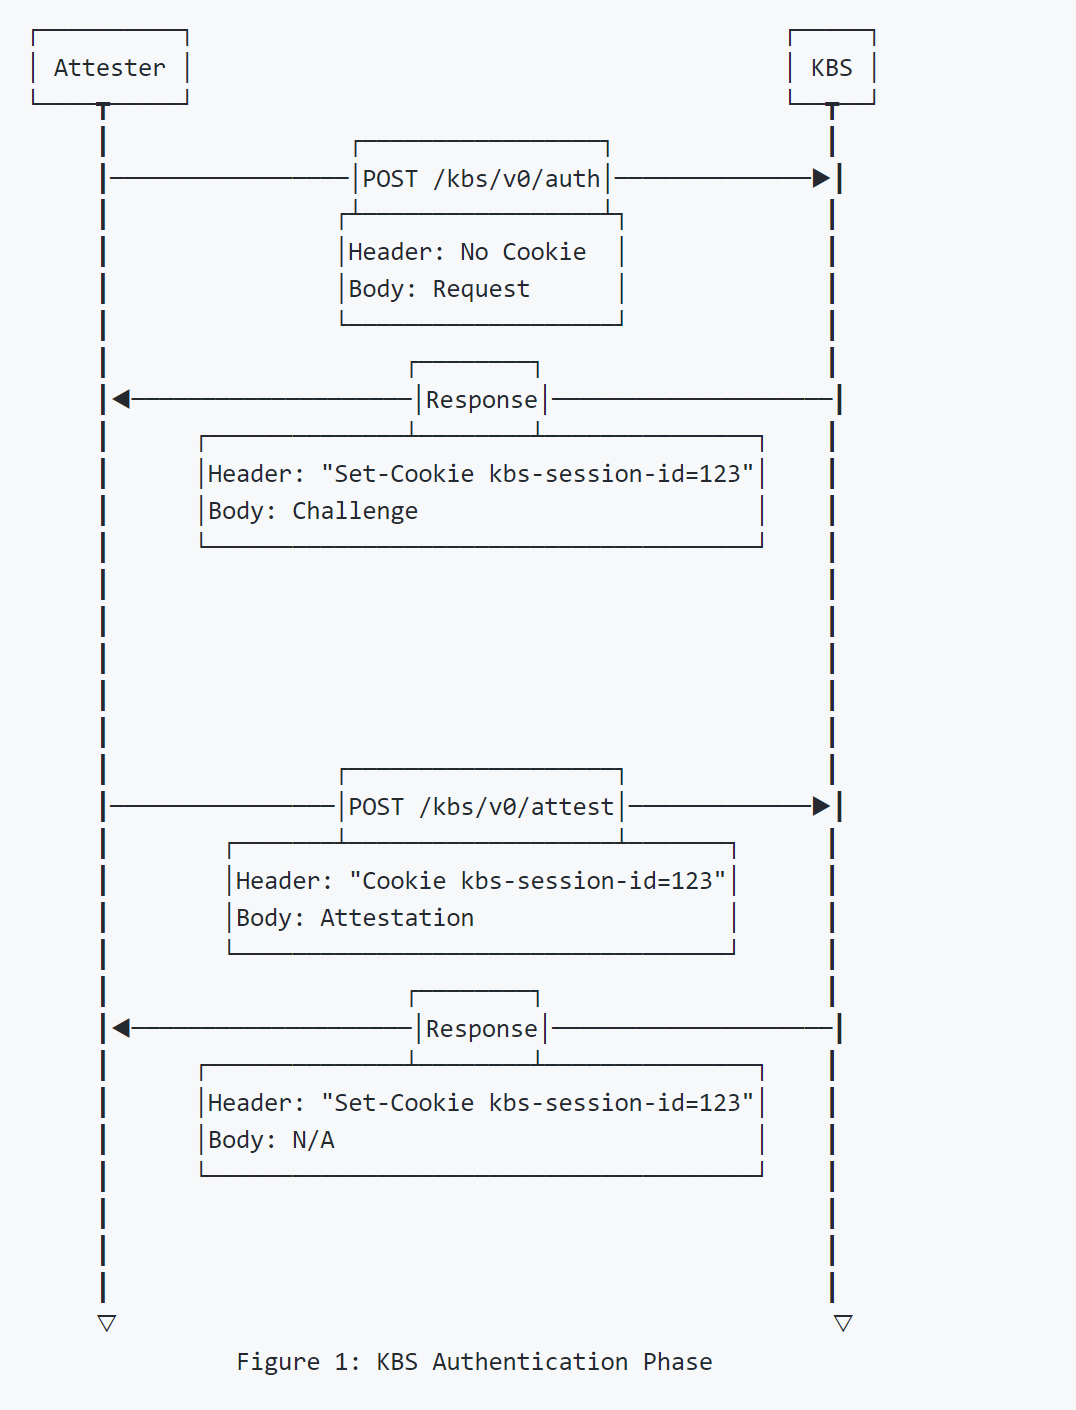
\includegraphics[width=0.8\textwidth]{images/attestation.PNG}
%     \caption[Authentication phase]{Authentication phase}
%     \label{fig:Authentication}
% \end{figure}

% As defined in Key Broke service attestation protocol, phase 1 (authentication phase) has 4 step: 
% \begin{displayquote}
%     \begin{enumerate}
%         \item  Request: The KBC sends the initial Request payload to the KBS, in order to authenticate itself against the KBS, and eventually request resources.
%         \item  Challenge: After receiving the initial Request payload, the KBS responds with the Challenge payload. This is how the KBS sends the attestation challenge to the KBC. Together with the attestation challenge, the KBS also sends a session identifier to the KBC, as an HTTP Cookie. This session identifier can be used to skip steps 2 and 3 after a successful attestation.
%         \item  Attestation: The KBC replies to the attestation challenge from step 2 with an attestation evidence, in order to prove that its environment (HW-TEE) is safe and reliable. The KBC sends an Attestation payload to the KBS, that contains the attestation evidence and the HW-TEE generated, ephemeral public key.
%         \item  Response: The KBS returns a Response payload to a KBC requesting a resource if and only if the Attestation payload was successfully validated. The KBC requests resources by sending HTTP GET requests to resource specific endpoints. Within the valid time of the HTTP Cookie generated by the KBS during step 2, the KBC can directly request resources or services from KBS, without going through steps 2 and 3.
%     \end{enumerate}
% \end{displayquote}

% \begin{figure}[H]
%     \centering
%     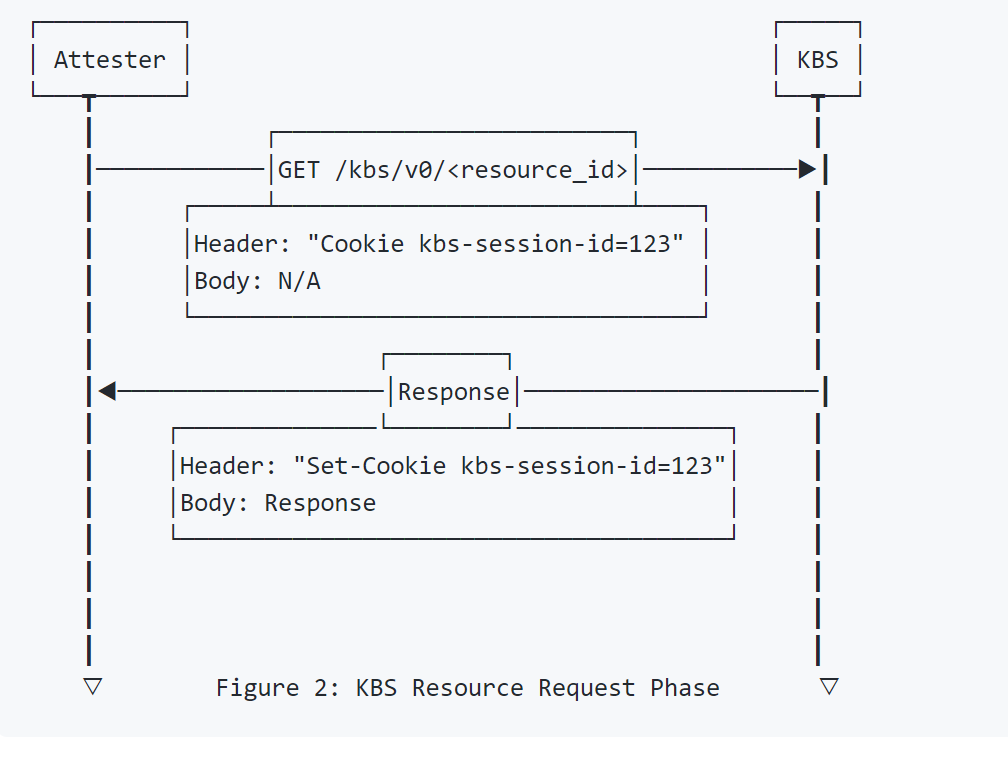
\includegraphics[width=0.8\textwidth]{images/resourcerequrie.PNG}
%     \caption[Resource Requests phase]{Resource Requests phase}
%     \label{fig:resourcerequrie}
% \end{figure}
% As defined in Key Broke service attestation protocol,  kbc can request resources or services from kbs during 2 phase in the following way:
% \begin{displayquote}
%     The KBS implementation keeps track of attestation results and binds them to a cookie identifier. During the second phase, the KBS can then decide if a specific resource could be released to a given attester, by mapping the cookie identifier the attester includes in 
%     its resource request message to its attestation results.

%     To request a protected resource from the KBS, the attester sends a GET request to a resource specific endpoint. If the attester is allowed to access the resource, the KBS will respond to the 
%     GET request with an HTTP response which content is set to a KBS Response JSON payload.
% \end{displayquote}

% \subsection{The whole procedure}
% \begin{itemize}
%     \item   The data owner generate a symitric key A and use it to encrypt file-related secrets.
%     \item  The data owner define the policy for qkernel shield, where the policy contains the key A, environment variable and arguments-related secret in plaintext, and the mount path of file-related secret.
%     \item  The data owner attests cas, and uploads the policy if the attestation succeeds.
%     \item  The data owner passed the encrypted file-related secret to cloud operator and the location to mount it, then informs cloud operator to create a confidential qkernel.
%     \item  The cloud operator then mounts the file-related secrets to the container's file system and starts the container. Note that the IP address of the CAS is passed to the container as an environment variable when the container is started.
%     \item  The shield inside the confidential qkernel then starts and sends the POD's attestation report to CAS via https.
%     \item  CAS verify the attestation report with the help of Intel/AMD remote attestation infrastructure. If the verification succeeds, CAS sends the policy file to the shield over https channel.
%     \item  Shield in turn loads the encrypted file-related secrets from the host, decrypts them, and keep them in the guest's memory. 
%     \item  Shield then reads the secrets related to environment variables and application arguments from the policy file and uses them as environment variables and  arguments for the application container process.
% \end{itemize}


% \section{Runtime issue}
% \subsection{Shared library loading during runtime}
% Motivation: Loading shared libraries during runtime may corrupt the container's confidential execution environment.
% For example, during container running, one issues the ls command to the container. After qkernel receives the command, qkernel finds the executable file "ls" in the /bin directory and creates a new process to execute the file. This process in turn loads shared library files from the host side, including ld-linux-x86-64.so.2, 
% libc.so.6,libpcre2-8.so.0, libdl.so.2, libpthread.so.0. These librarys may contain vulnerable gadgets that could be used in spectre attack.
% Since such side channel attack is caused by hardware vulnerability, most hardware based TEEs can not protect the workload from it. Therefore, this could lead an Adversary to exploit vulnerabilities in the shared libraries to attack containers running in the confidential qkernel.

% Mitigation: Shiled checks the libraries' signatures using the signer's public key obtained from the policy file before loading them into guest memory. Note that it is assumed that the signer has performed a security audit on the signed library to ensure that there are no vulnerabilities in the library files.

% \subsection{volume managed by k8s}
% \label{volume_managed_by_k8s}
% Motivation: Applications that require storage may write their secrets to k8s managed volumes.
% Nowadays, many applications require the use of disks to store non-volatile data. Such applications include various database applications. Thereby, to facilitate these applications to run in the cloud, cloud providers offer various storage services, 
% the most notable of which is Amazon Simple Storage Service (S3). In the context of k8s, these storage services are also uniformly referred to as volume. One can create a volume object of arbitrary size and mount it to a specified path in the container file 
% system when creating the container. This is super convenient in terms of deployment. However, since the volume is provided by the cloud provider, any data stored on the volume is at risk of being compromised. To this end, we must find a way to use volumes while protecting 
% the confidentiality of the data.

% Mitigation: The idea is straightforward: the shield should encrypt the data before it is written out of the confidential qkernel and decrypt the data read into the confidential qkernel from the host. 

% \begin{figure}[H]
%     \centering
%     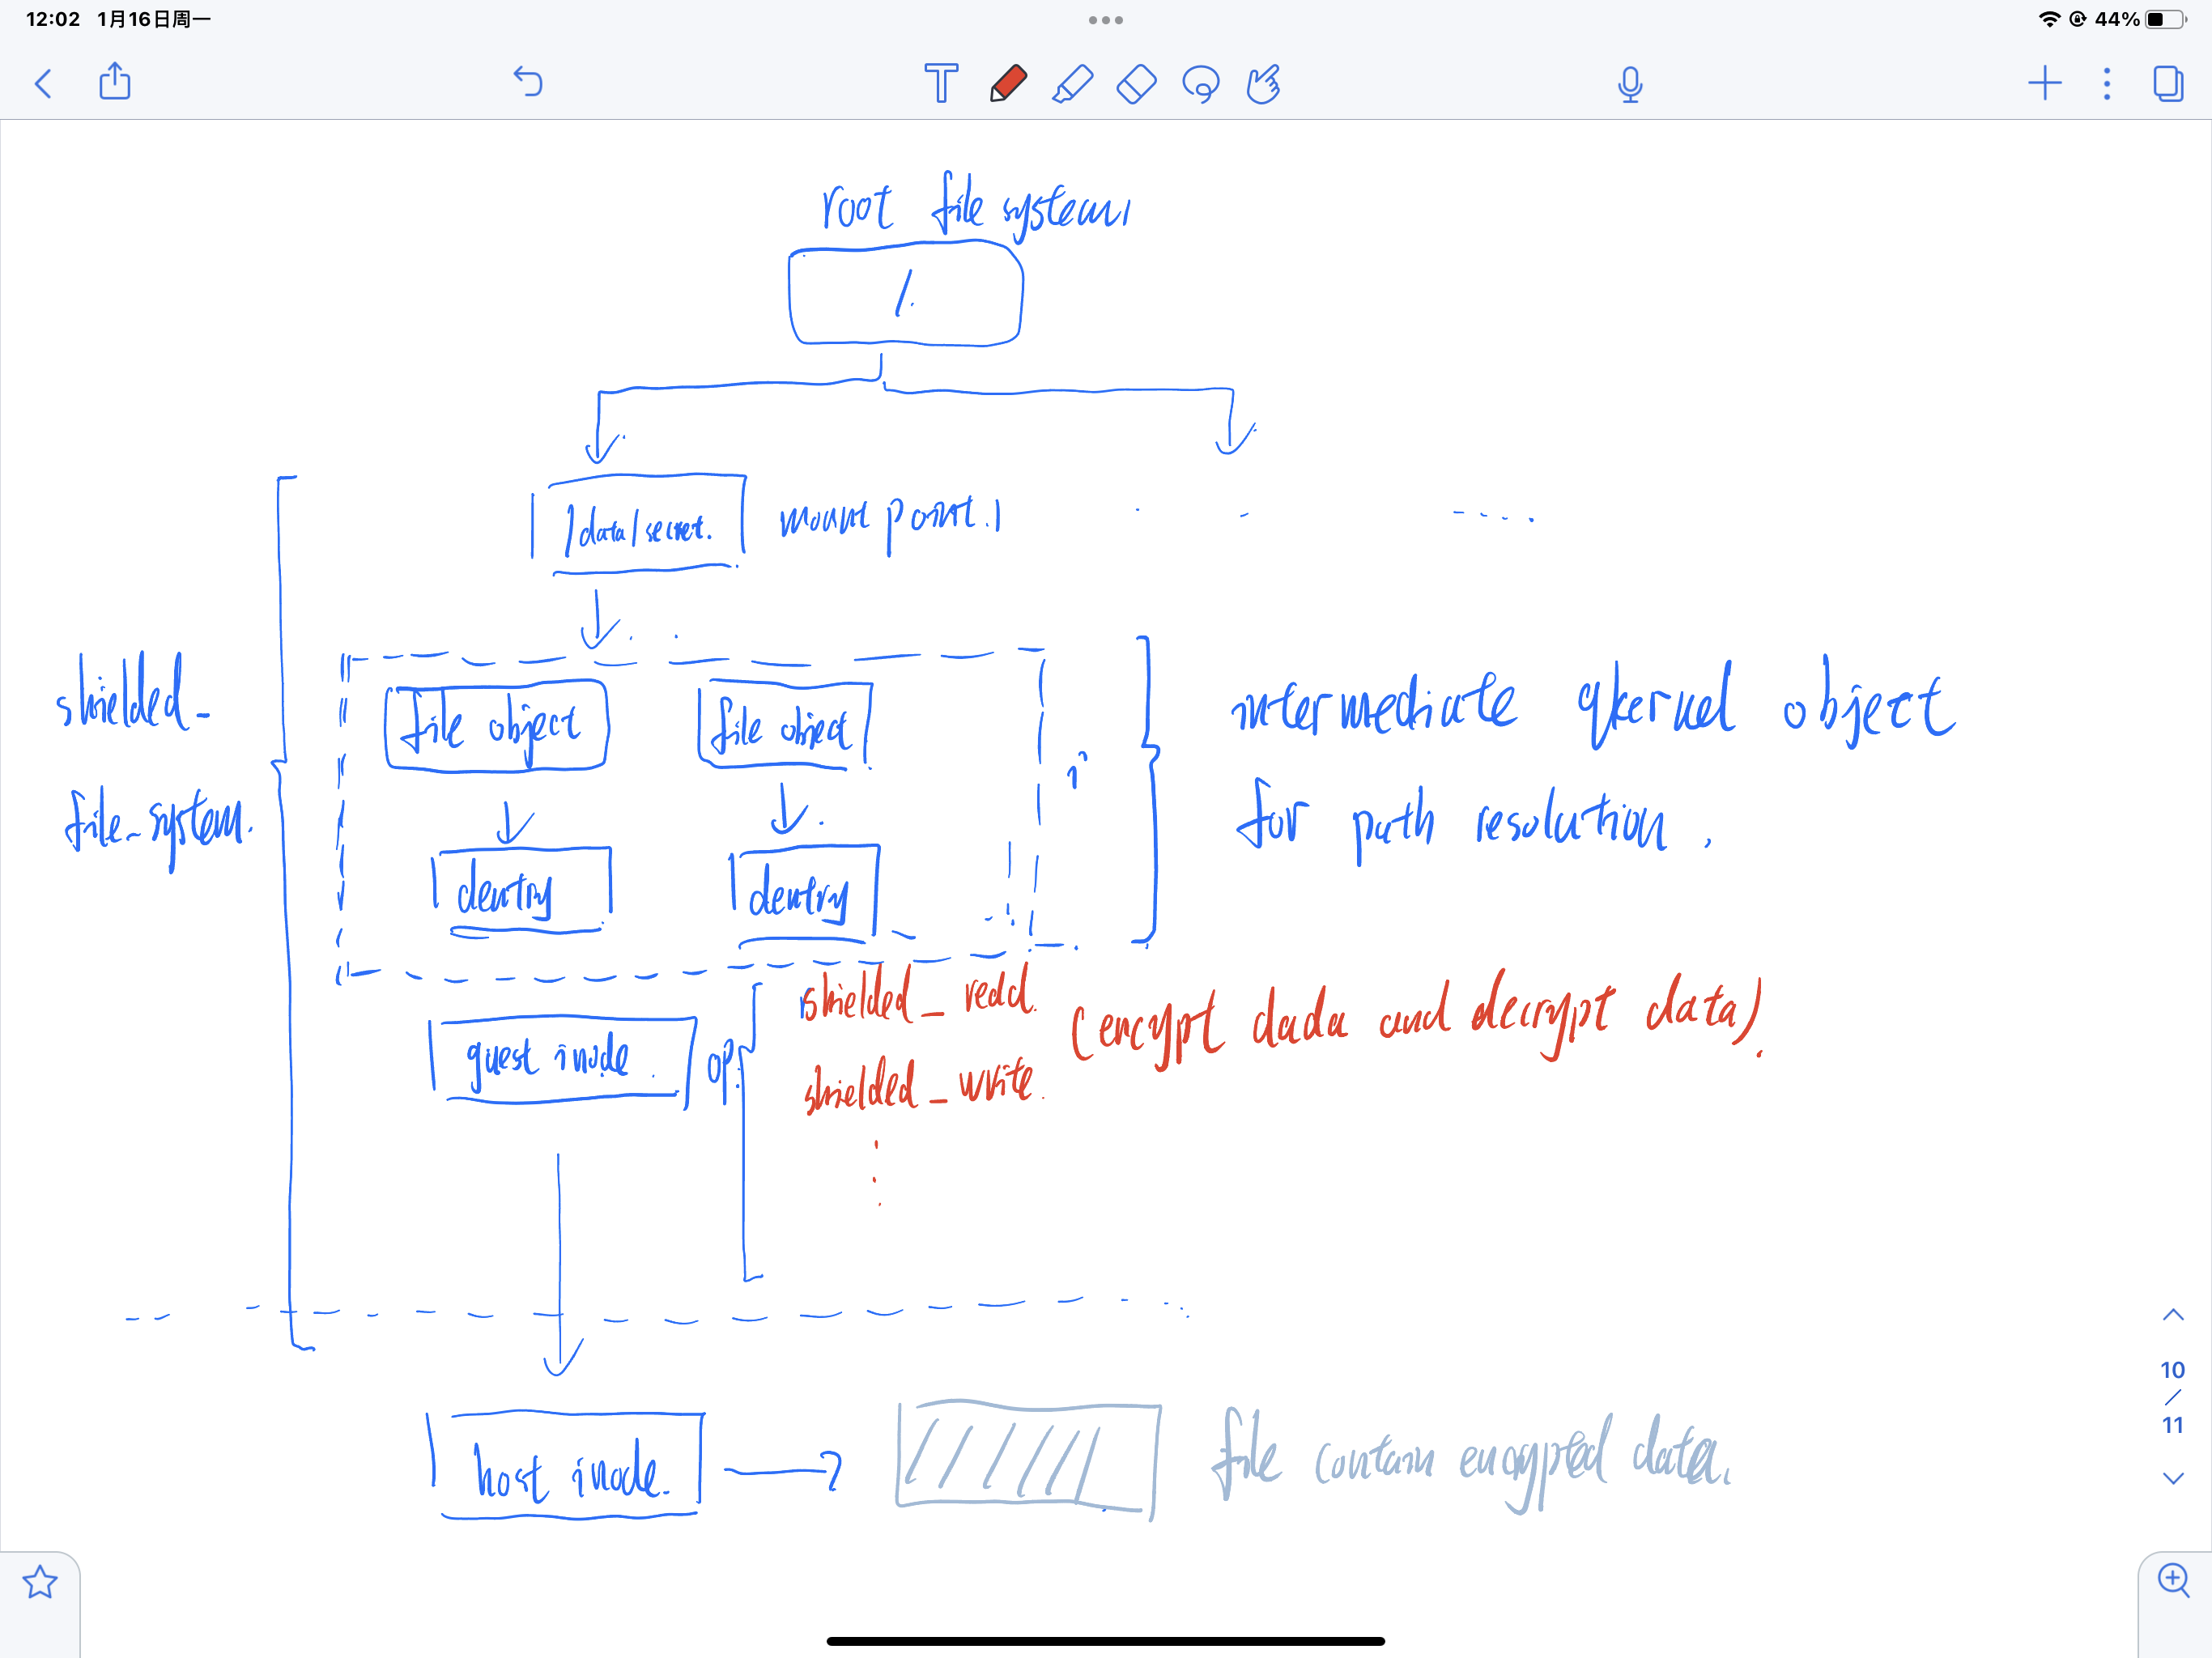
\includegraphics[width=0.8\textwidth]{images/IMG_4413.PNG}
%     \caption[shielded file system]{shielded file system}
%     \label{fig:shielded_filesystem}
% \end{figure}
% Since we only want to protect the data written to the volume mounted to a specific path rather than encrypting the entire filesystem, we have to solve the file path resolution issue, which includes the 
% resolution of hard links, soft links, and relative and absolute paths. To avoid developing complex path resolution algorithms and to maximize the reuse of the existing filesystem infrastructure in the qkernel, we create a new filesystem type, the "shield filesystem," on 
% the mount path of the volume and reuse the qkernel objects such as file, dentry, and inode.

% In the diagram, we assume that the volume is mounted to the /data/secret directory of the container filesystem. During container initialization (during start container req), shield will mount the shield filesystem on this path. This filesystem is located in the qkernel and 
% uses the existing filesystem objects in the qkernel, i.e. "file," "dentry," to resolve the file path. After completing the path resolution, a function defined in the inode operation list will be triggered. In the case of a write-request, the shielded\_write function will be called.
% shielded\_write function uses the file system encryption key to encrypt the data and protect the integrity of the data. The encrypted data is then written to the volume on the host machine.

% \begin{figure}[H]
%     \centering
%     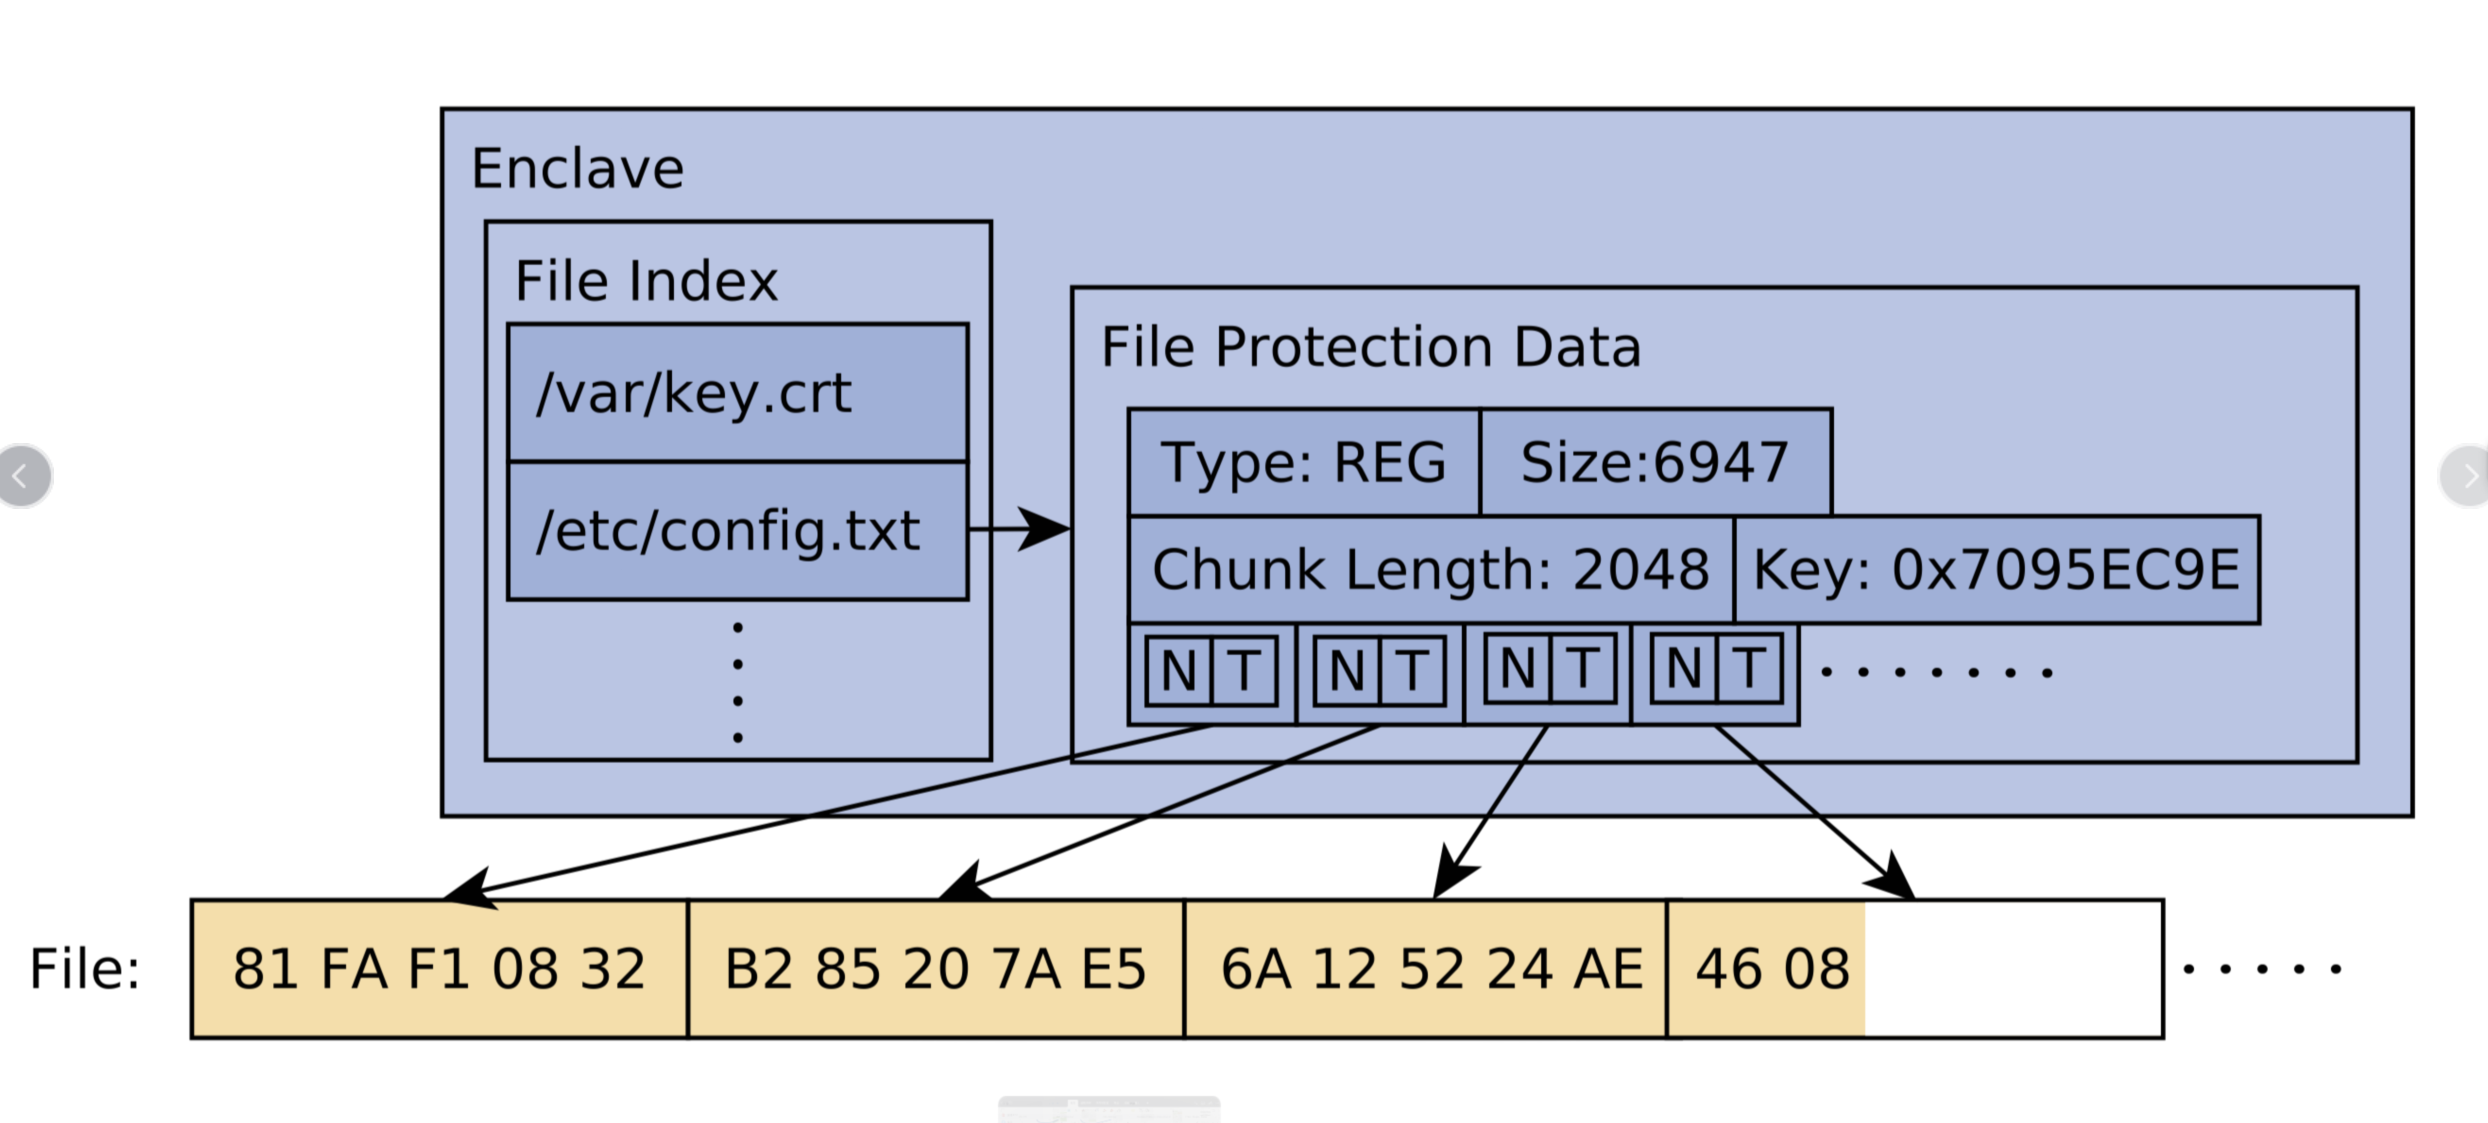
\includegraphics[width=0.8\textwidth]{images/fileencption.png}
%     \caption[file content encryption]{file content encryption}
%     \label{fig:file_content_encryption}
% \end{figure}
% Encrypting the contents is done by querying the shield-preserved data structure using a unique inode id. shield preserves a file protection data structure for each inode in the shielded file system. This structure contains the various metadata needed by shielded\_write/shielded\_read to encrypt and 
% decrypt the file. This metadata comprises a list of nonces, an authentication tag for each individual chunk, the size of the file, etc. Because each inode has a unique id, the shielded\_write/shielded\_read functions can easily find the structure corresponding to an inode.
% When shielded\_read is called, it requests the file content from the host in a chunked fashion and performs the necessary authentication checks before the decryption. This chunk-wised protection mechanism may add certain overhead to the file access in case the file access does not 
% coincide with the chunk boundary.




% \subsection{There may be more issues}
% \subsubsection{Shared memory}
% \subsubsection{Message queue}

% \section{Endpoints related}
% \subsection{Overview of endpoints defined in CRI runtime service}
% \begin{itemize}
%     \item  attach:Attach to a running container
%     \item  exec:Run a command/termianl in a running container
%     \item  logs: Fetch the logs of a container
%     \item  port-forward: Forward local port to a pod

%     \item  inspect: Display the status of one or more containers
%     \item  inspectp: Display the status of one or more pods
%     \item  ps:  List containers
%     \item  pods: List pods
    
%     \item  create: Create a new container
%     \item  start: Start one or more created containers
%     \item  run:Run a new container inside a sandbox
%     \item  runp:Run a new pod
%     \item  rm:Remove one or more containers
%     \item  rmp:Remove one or more pods
%     \item  stop:Stop one or more running containers
%     \item  stopp: Stop one or more running pods

%     \item  update: Update one or more running container's resources (CPU, memory etc.)
%     \item  stats: List container(s) resource usage statistics
%     \item  statsp: List pod resource usage statistics
% \end{itemize}

% All endpoints can be classified into four categories according to their usage:
% \begin{itemize}
%     \item  Debug-purpose endpoints:attach, exec, logs, port-forward:
%     \item  Endpoints for Pod/container lifecycle management: create, start, run, runp, rm, rmp, stop, stopp
%     \item  Endpoints for collecting container/pod metadata stored in high level container runtime: inspect, inspectp, ps, pods
%     \item  Endpoints for Pod/container raw resources management (cpu, memory, etc.,): update, stats, statsp
% \end{itemize}

% Conclusion.
% \begin{itemize}
%     \item  The debug-related endpoints can be exploited by malicious attackers and compromise confidential qkernel. Thus we analyze these endpoints in detail in the later sections
%     \item  Endpoints about container lifecycle management do not reveal any secret, but we have to consider 2 cases:
%     \begin{itemize}
%         \item  For the start container req from start endpoint, we have to consider how to pass secrets to the legacy application container----> solution: see section \ref*{Secure_deployment} "secure deployment“
%         \item  When the start container req reaches the shim process, the shim process may mount the k8s managed volume, this means during runtime an application may write secrets to the cloud provider managed volume ----> solution: need shield file system, see section \ref*{volume_managed_by_k8s} "volume managed by k8s"
%     \end{itemize}
%     \item Endpoints for collecting container/pod metadata stored in high level container runtime do not reveal any secrets kept in confidential qkernel. Because requests from these Endpoints only collect container/pod metadata stored in high level container runtime (conainerd), i.e. these requests are not sent to the confidential qkernel
%     \item  Endpoints for Pod/container raw resources management: does not reveal any secrets stored in the confidential qkernel, because these Endpoints only collect the use of raw resources by the confidential qkernel.
% \end{itemize}


% \subsection{Exec endpoint}
% \subsubsection{Terminal mode(done)}
% We provide option in policy to disable the termianl mode
% However, it is important to note that the confidential qkernel does not protect the stdin/out of the terminal when terminal allocation is allowed. 

% The reason is that we argue that terminal allocation should be rejected in production, i.e., termianl should only be used in the development phase. In a multi-stakeholder scenario, secrets may come from different stakeholders. When one stakeholder 
% gains access to the container through terminal, the confidential qkernel cannot restrict that stakeholder from reading the secrets of other stakeholders. More specificlly, when the qkernel receives a terminal allocation request, it starts a process 
% that executes the /bin/sh executable. The commands sent by the stackholder to the container through the termianl will be executed by this process. Since the process is running inside the confidential guest, the guest's memory, the cpu registers being 
% used, and the files in the container file system are all in plaintext to the process. So the process can read the others secrets and return it to the stakeholder.

% In a production environment, if one wants to send commands to a container running under the protection of the confidential qkernel, he should use the Single cmd line mode. In this mode, the qkernel allows one to send a request each time to the container to execute a command. 
% When the qkernel receives the request, the qkernel whether the issuer has permission to execute the command by reading the policy file. In this way, we effectively avoid secrets disclosure in multi-stakeholder
% scenarios.

% \subsubsection{Single cmd line mode(done)}
% In this mode, the qkernel allows one to send a request each time to the container to execute a command. 
% When the qkernel receives the request, the qkernel checks whether the issuer has permission to execute the command by reading the policy file.

% In mode, qkernel adopts the role based access control mechanism, and defines for each role the commands it can execute and the directories in which these commands can be executed. 
% The following figure shows a fragment of the policy file. In this policy, we have defined three roles: data owner, code owner, and host (cloud provider). The host role, for example, is allowed 
% to execute cat and ls commands in the /var directory and its subdirectories. If the host sends a request to the container to execute command not defiend in the policy, the qkernel will refuse 
% to execute the request.
% \begin{lstlisting}[language=json,firstnumber=1]
%     {
%         "singleShohCommandLineModeConfigs": [
%             {   
%                 "role": "DataOwner",
%                 "allowedCmd": ["cat", "ls", "cd", "rm",],
%                 "allowedDir": ["/usr/data_owner/"]
%             },
%             {   
%                 "role": "CodeOwner",
%                 "allowedCmd": ["cat", "cp"],
%                 "allowedDir": ["/usr/code_owner/"]
%             },
%             {   
%                 "role": "Host",
%                 "allowedCmd": ["cat", "ls"],
%                 "allowedDir": ["/var"]
%             }
%         ]
    
    
%     }
% \end{lstlisting}



% \subsubsection{How qkenel identify the request issuer}
% \begin{itemize}
%     \item  cmd issuer first require an access token from CAS, this access token contain the request information and the role of the cmd issuer
%     \item  cmd issuer then send the encrypted request along with the access token to qkernel through the k8s channel
%     \item  qkernel verifies the token by sending it to CAS. If the token is valid, CAS sends a HTTP response that contains the "true" keyword and other related information
%     \item  qkernel finaly exec the cmd according to the policy defined for the role
% \end{itemize}
% \subsubsection{How to prevent the host from viewing the request contents (cmd and its associate arguments), as well as the request result}
% The request itself and its execution results are encrypted and integrity-protected using AES-GCM.

% \subsection{Log endpoint (done)}
% Logs streaming from the container's stdout/err are encrypted and integrity-protected using AES-GCM.
% \subsection{Attach endpoint}
% Since the stdout/err of the container is encrypted, a client without the decryption key cannot get any useful data through the channel established by the Attach endpoint.

% \subsection{Port-forward endpoint}
% Port-forward endpoint is out of scope

% \section{Secure Client(in theory)}

% \begin{itemize}
%     \item  Prepare the policy and secrets including:
%     \begin{itemize}
%         \item  encrypts the file-related secrets using key A (File-related secret encryption key)
%         \item  requests the cloud operator to mount the encrypted secret to a certain path
%         \item  embeds key A  and the mount path to policy so that qkernel can find and decrypt it.
%         \item  Add arguments and environment variable-related secrets to the policy file
%     \end{itemize}
%     \item Attest the CAS and upload the policy
%     \item  Get access token from CAS, encrypt the Single cmd line mode request, and decrypt its result using "Exec request and result encryption key"
%     \item  decrypt the container's log using the "Log encryption key" got from cas
%     \item  issue dynamic attestation request to qkernel
% \end{itemize}


% \section{Keys}

% \begin{itemize}
%     \item  File-related secret encryption key (symmetric): each role possesses its own key for file-related secret encryption. It is generate by role and loaded to qkernel through a secure channel for file-related secret decryption.
%     \item  File system encryption key (symmetric): the key is used for encrypting files in the shield file system. It is generated by CAS and transmitted to confidential qkernel through a secure channel.
%     \item  Exec request and result encryption key (symmetric): each role possesses its own key for encrypting the exec req (for example, the command and its arguments).  It is generate by role and loaded to qkernel through a secure channel for decrypting the exec request and encrypting the result of the exec request.
%     \item  Indentification key of CAS(asymmetric): The public part of the key is transmitted to qkernel in a effenciant way.  This public key allows the qkernel to validate the identity of the CAS during the HTTPS (tls) handshake, thus effectively preventing an adversary from hijacking the CAS address to masquerade as a CAS and spoof the qkernel.
%     \item  Log encryption key (symmetric): This key is generated by CAS and loaded into qkernel via a secure channel. it is used by qkernel to encrypt the logs coming out of the container's stdout/err stream. A trusted client with appropriate privileges can obtain the key from cas and decrypt the logs.
% \end{itemize}
\cleardoublepage

%%% Local Variables:
%%% TeX-master: "diplom"
%%% End:
